\chapter{Appendix}\label{ch:appendix}

% @formatter:off
\begin{listing}[h!]
    \centering
    \begin{minted}[autogobble,breaklines=true]{shell}
        $ curl --location 'localhost:9000/compute' \
        --header 'Content-Type: application/json' \
        --data '{
            "instanceParameters": {
                "layout": {
                    "width": 30,
                    "height": 20,
                    "evalFunc": "f(x,y) = x+y"
                },
                "paintings": [
                    { "ident": "1", "width": 5, "height": 7 },
                    { "ident": "2", "width": 5, "height": 7 },
                    { "ident": "3", "width": 5, "height": 7 },
                    { "ident": "4", "width": 5, "height": 7 },
                    { "ident": "5", "width": 5, "height": 7 },
                    { "ident": "6", "width": 5, "height": 7 }
                ],
                "paintingsFlow": [
                    { "from": 1, "to": 2, "flow": 3.3 },
                    { "from": 1, "to": 3, "flow": 4.4 },
                    { "from": 1, "to": 5, "flow": 0 }
                ]
            },
            "gaParameters": {
                "maxNumberOfIter": 300,
                "populationSize": 300,
                "maximumWildCardCount": 1,
                "orientationWeights": [ 1, 1, 0.5 ],
                "geneticAlgorithm": "simpleGa",
                "mate": "normalizedProbabilityVectorSum",
                "mutate": "flipOnePartAtRandom",
                "select": "tournament",
                "objective": "simple",
                "evaluator": "ga",
                "placingHeuristics": "corner",
                "populationDivisionCounts": {
                    "elite": 0.2, "average": 0.6, "worst": 0.2,
                    "children": 0.3, "mutant": 0.2, "winner": 0.2,
                    "random": 0.1
                },
                "initialPopulationDivisionCounts": {
                    "random": 0.7, "greedy": 0.3
                }
            },
            "objectiveParameters": {
                "name": "simple",
                "params": {
                    "overlappingPenalizationConstant": 36.05,
                    "outsideOfAllocatedAreaPenalizationConstant": 36.05
                }
            }
        }'
    \end{minted}
    \cprotect\caption[Example of computation submission without instance name]
    {Example of computation submission using \verb|curl|\footnote{\url{https://curl.se/}} without specifying the instance name.
    Without it, everything has to be entered manually into the request – layout width and height, paintings together with their flow, and evaluation function.
    }

    \label{lst:computation-submission-manual}
\end{listing}
% @formatter:on


\afterpage{%
    \clearpage% Flush earlier floats (otherwise order might not be correct)
    \begin{landscape}% Landscape page
        \begin{figure}
            \centering
            \subfloat{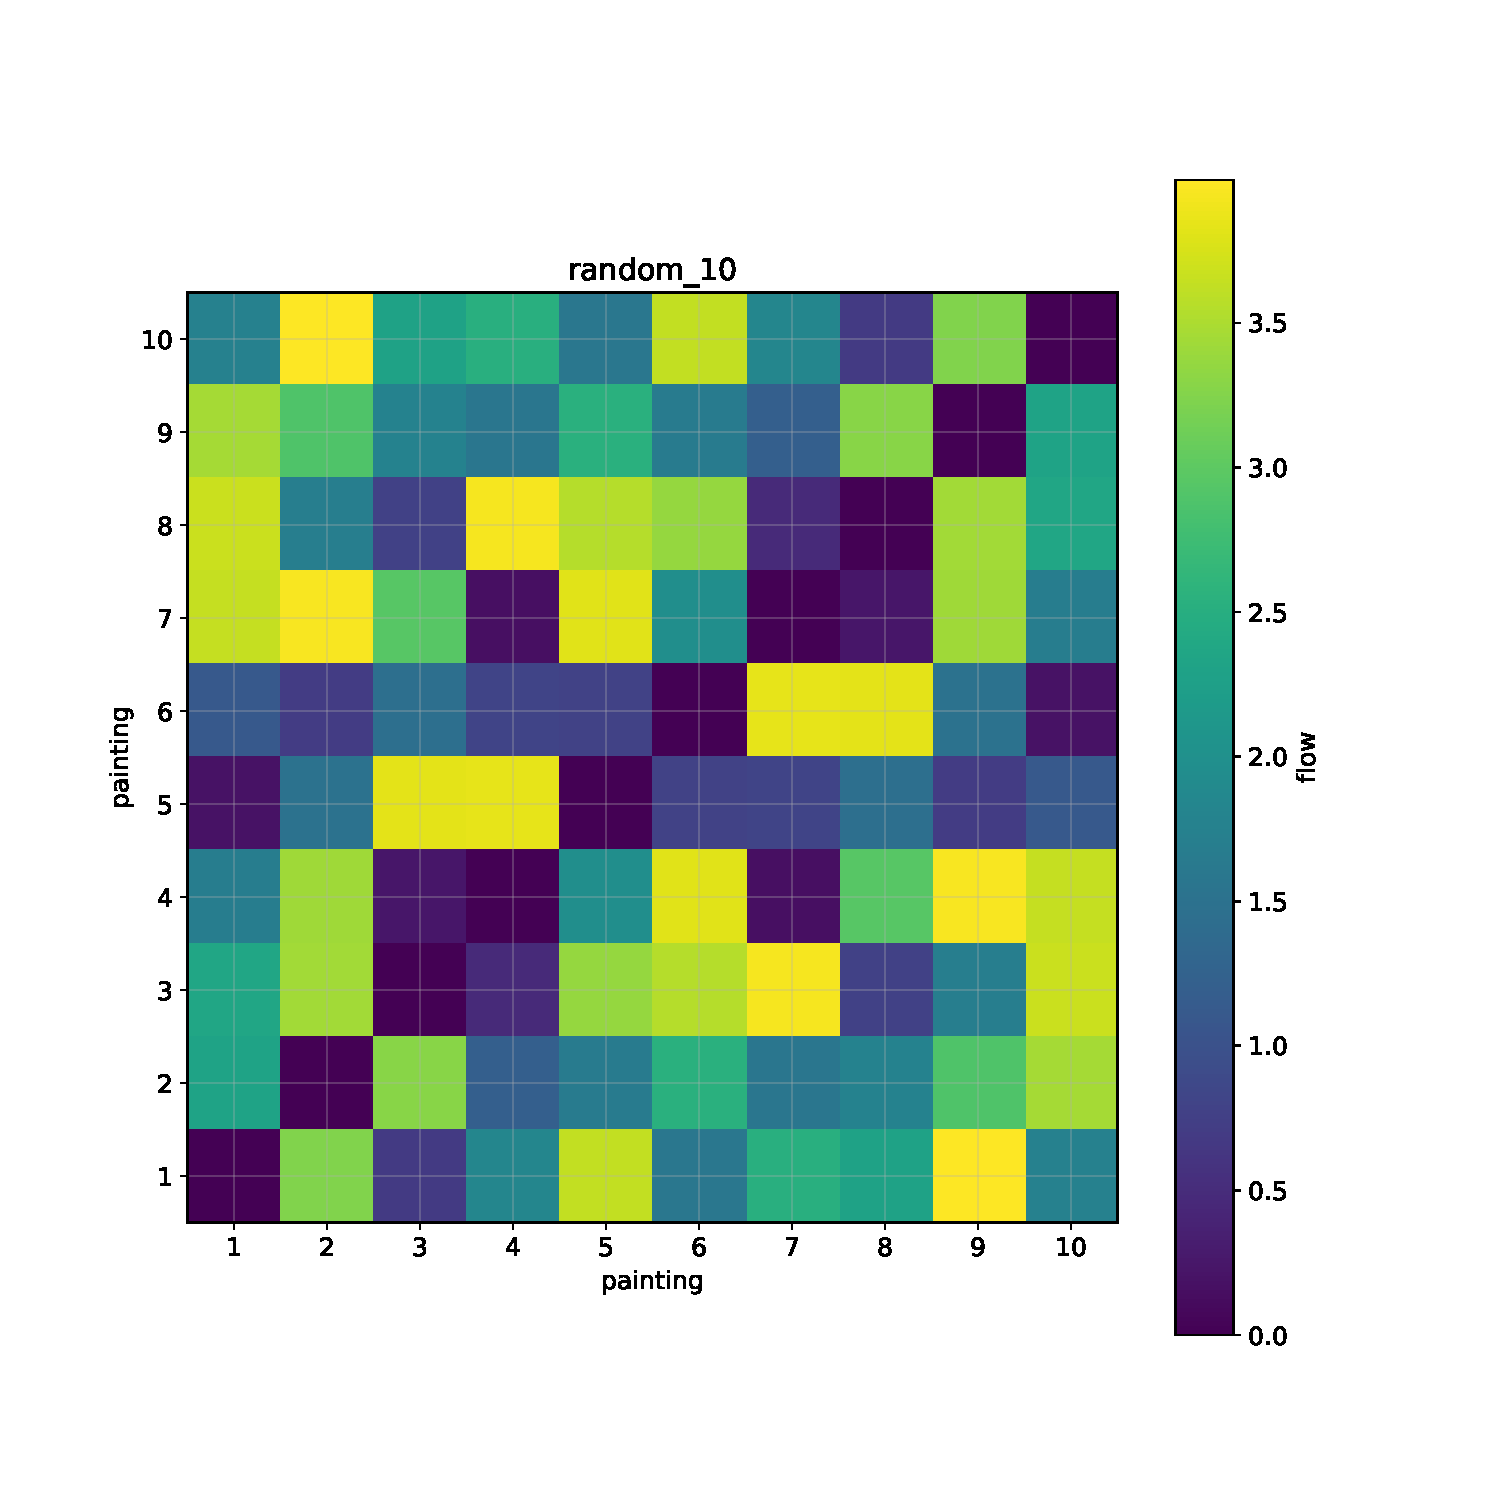
\includegraphics[width=0.8\textwidth]{heatmap_random_10}\label{subfig:heatmap-random-10}}
            \subfloat{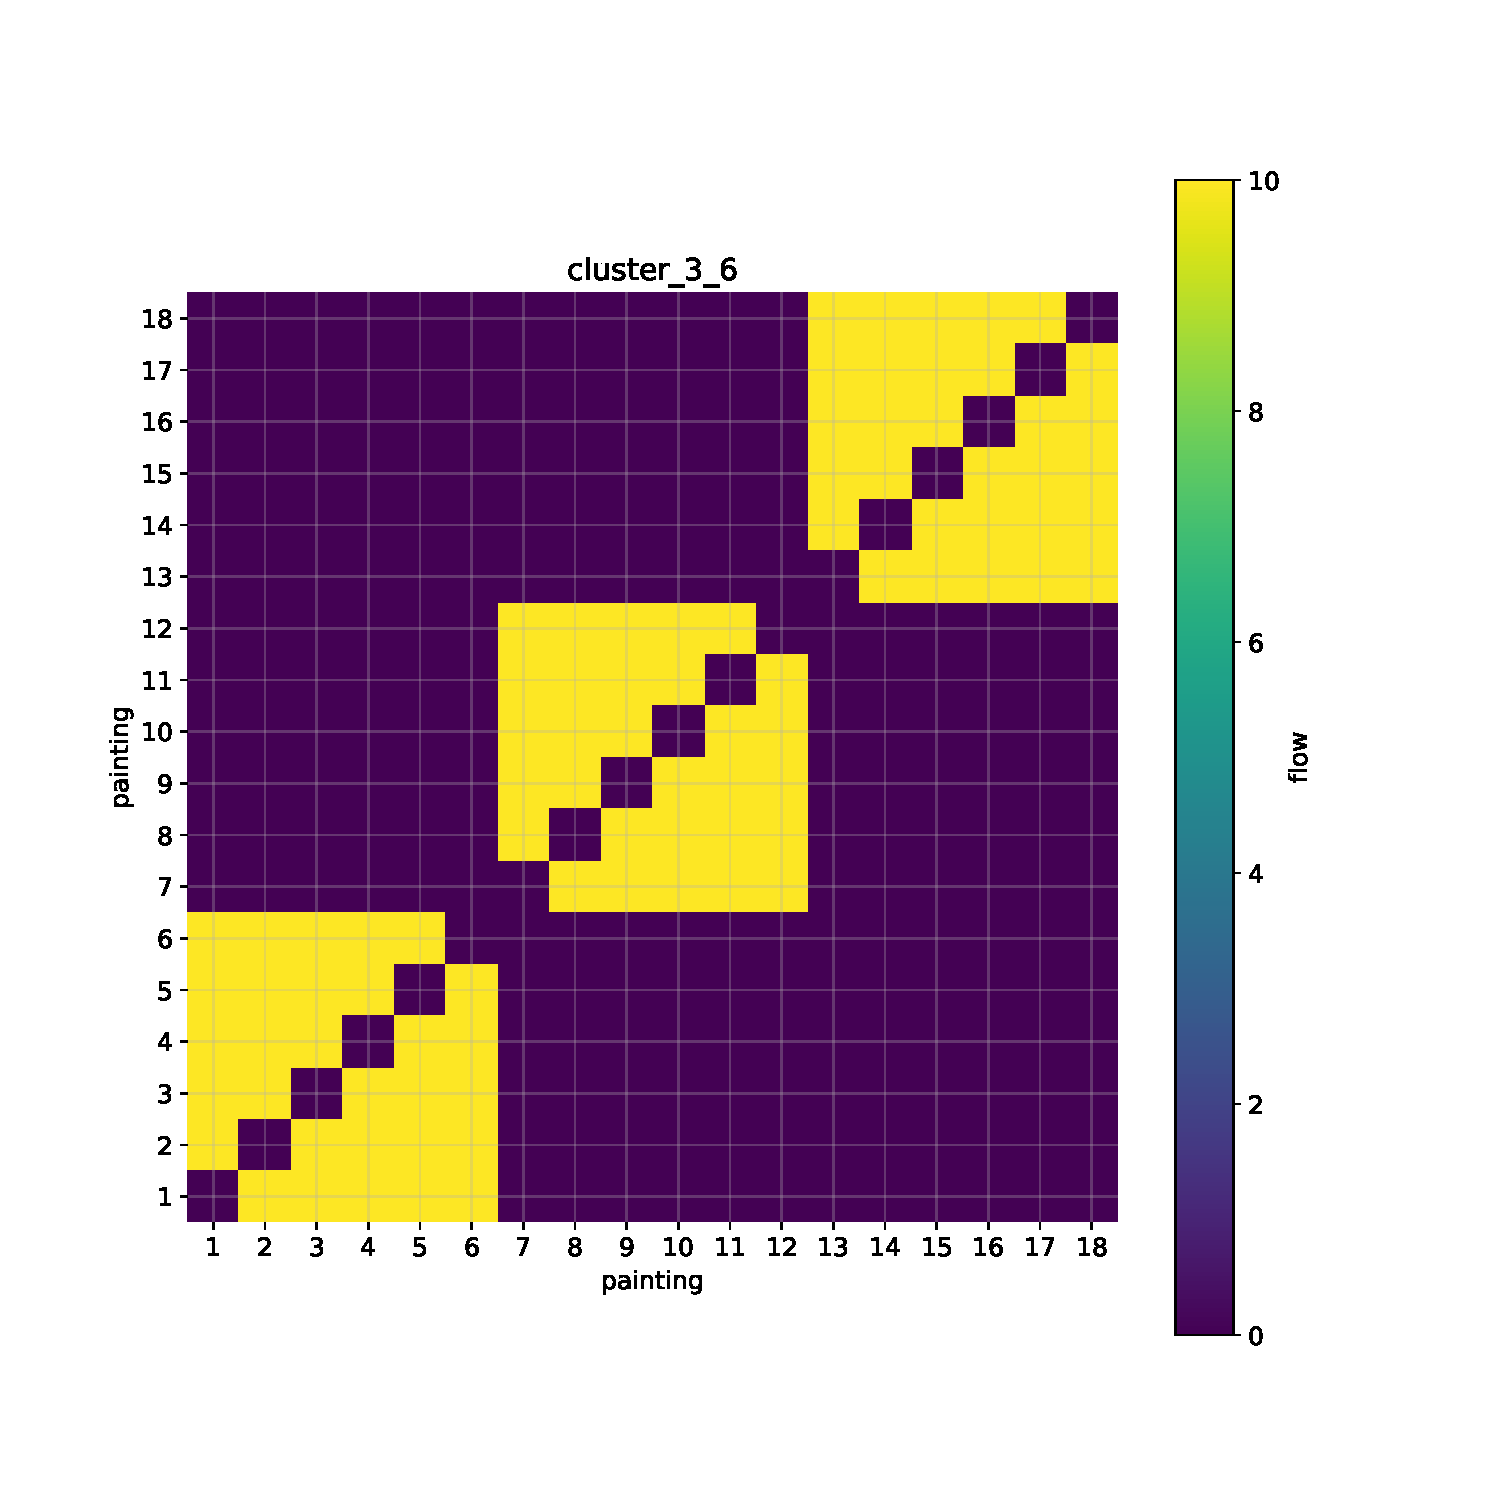
\includegraphics[width=0.8\textwidth]{heatmap_cluster_3_6}\label{subfig:heatmap-cluster-3-6}}
            \caption[Flow visualization examples]
            {Visualization of the flow for two painting placement instances. Flow expresses the affinity of paintings to each other.
            Paintings that should be placed close together have flow higher compared to paintings
            that should not.
            Flow matrices are symmetric,i.e., the flow between two paintings is the same from each direction. Also, the flow to/from itself is zero.
            }
            \label{fig:instance-flow}%
        \end{figure}
    \end{landscape}
    \clearpage% Flush page
}